\section{Lab 2 - Latches, Flip-Flops, and Counters}

\subsection{Introduction}
Elementary latches and flip-flops have been used for years as a means to store temporary data either from the outputs of logic operations or by setting them to configure logic to behave in certain ways. This lab will go into the aspects of creating latches and flip-flops which will then be used to create a counter. 

\subsection{Pre-lab}
Before you begin this lab you should complete the following and upload to Sakai:

\begin{itemize}
	\item Write down the truth table for a D-latch, SR-latch and J-K flip-flop
	\item Design a block diagram for an 8-bit synchronous counter using J-K flip-flops
\end{itemize} 

\subsection{Lab Activities}

\subsubsection{Latches}
The following VHDL code implements the logic for a D-latch based off of the schematic in Figure \ref{fig:dlatch}. 

\begin{lstlisting}
-- A gated D latch
LIBRARY ieee;
USE ieee.std_logic_1164.all;

ENTITY dlatch IS
	PORT (	CLK, D	: IN	STD_LOGIC;
		Q, Qbar	: OUT	STD_LOGIC);
END dlatch;

ARCHITECTURE rtl OF dlatch IS

	SIGNAL D1, D2, Qa, Qb : STD_LOGIC; -- Intermediate signals
	ATTRIBUTE keep: boolean; -- For waveform results
	ATTRIBUTE keep of D1, D2, Qa, Qb : signal is true;
	
BEGIN
	
	D1 <= NOT (D AND CLK);
	D2 <= NOT (D1 AND CLK);
	Qa <= NOT (D1 AND Qb);
	Qb <= NOT (D2 AND Qa);

	Q <= Qa;
	Qbar <=Qb;
	
END rtl;
\end{lstlisting}


\begin{figure}[H]
	\centering
	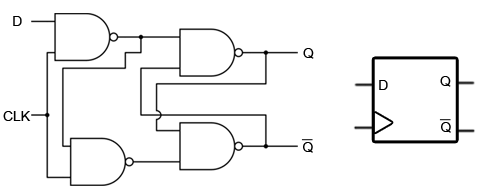
\includegraphics[width=100mm]{Lab2/figures/dlatch.png}
	\caption{D-latch circuit and block diagram}
	\label{fig:dlatch}
\end{figure}

Using this as a reference, design VHDL for an SR-latch with a clock input. Verify with waveforms that the circuit behaves the same as the truth table you created in the pre-lab.


\subsubsection{Flip-Flop}
Design VHDL code that implements the logic for a J-K flip-flop from Figure \ref{fig:jkflipflop}. Verify with waveforms that the circuit behaves the same as the truth table you created in the pre-lab 

\begin{figure}[H]
	\centering
	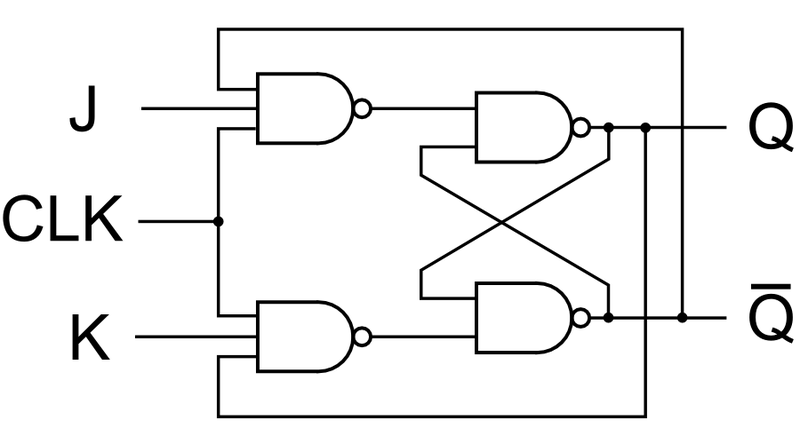
\includegraphics[width=100mm]{Lab2/figures/jkflipflop.png}
	\caption{J-K fip-flop circuit}
	\label{fig:jkflipflop}
\end{figure}

\subsubsection{Counters}
In the pre-lab, you created a block diagram for an 8-bit counter using J-K flip flops. Using the same VHDL code you created for implementing the J-K flip-flop, implement an 8-bit counter that increments when you press KEY0 on the DE2-115 development board. Link the binary output of the flip-flops to the red LEDs and then convert the binary value into hexadecimal to be shown on the 7-segment displays. \emph{Hint: you should refer to your code for the 7-segment display driver designed in the previous lab.}

\subsection{Lab Report}
Your lab report submission should break down as follows:
\begin{itemize}
	\item Extract from the fpga lab folder the VHDL file from each project, upload each of them to the Sakai Assignment page. Ex: part1.vhdl and part2.vhdl
	\begin{itemize}
		\item Make sure that your code is well commented.
	\end{itemize}
	\item Waveforms for the SR latch and JK flipflop (if JK doesn't work, try implementing it as a truth table with if statements)
	\item For Part 3 after compilation go to Tools > Netlist Viewers > RTL Viewer. Print a pdf of this page and discuss what you see.
	\item In a separate txt or pdf document, prepare a discussion on your compilation results. Be sure to include specifics about the amount of hardware used and where the numbers in the compilation results came from. Do the numbers make sense? Why? How do these results impact the use of FPGAs in industry? This should be no more than one page long, less is preferred.
\end{itemize}
